\documentclass[12pt]{amsart}
\usepackage{amsmath,amssymb}

\usepackage[usenames,dvipsnames]{color}
\usepackage[margin=1.25in]{geometry}
\usepackage{hyperref}
\usepackage{algpseudocode}
\usepackage{graphicx}
%\usepackage{tikz}

\newtheorem{theorem}{Theorem}[section]
\newtheorem{lemma}[theorem]{Lemma}
\newtheorem{proposition}[theorem]{Proposition}
\newtheorem{corollary}[theorem]{Corollary}
\newtheorem{claim}[theorem]{Claim}

\theoremstyle{definition}
\newtheorem{definition}[theorem]{Definition}
\newtheorem{notation}[theorem]{Notation}
%
\theoremstyle{remark}
\newtheorem{remark}[theorem]{Remark}
\newtheorem{example}[theorem]{Example}

\newcommand{\cat}[1]{\mathbf{#1}}
\newcommand{\eps}{\varepsilon}
\newcommand{\R}{\mathbb{R}}
\newcommand{\Z}{\mathbb{Z}}
\newcommand{\N}{\mathbb{N}}
\newcommand{\norm}[1]{\lVert#1\rVert}

\begin{document}

In order to create a bifiltered Rips complex from a set of points that is parameter-free, we must be able to account for simplices to be multi-critical. We say that a $k$-simplex, a subset of $k$ distinct points, appears at a pair $(a, b)$, if in the full set of points we connect any two points where $d(x, y) \le b$, the $k$ simplex is complete and each vertex has degree $\ge a$. So we see that putting the inverted ordering of $\R$ on the $x$-axis and the regular ordering on the $y$-axis, that if the simplex appears at a point $(a, b)$, then it appears at all points $(c, d) \ge (a, b)$, where $c \le a$ in the usual ordering. Thus, if we graph all the points of appearance of a simplex, we will see a staircase shape. Note that since the degree of a vertex of discrete and there exists a maximal degree (the total number of vertices), this staircase will be finitely generated. So, the grades of appearances of a multi-critical simplex in this form can be succinctly represented as a finite set of incomparable points.

\begin{figure}
	\centering
	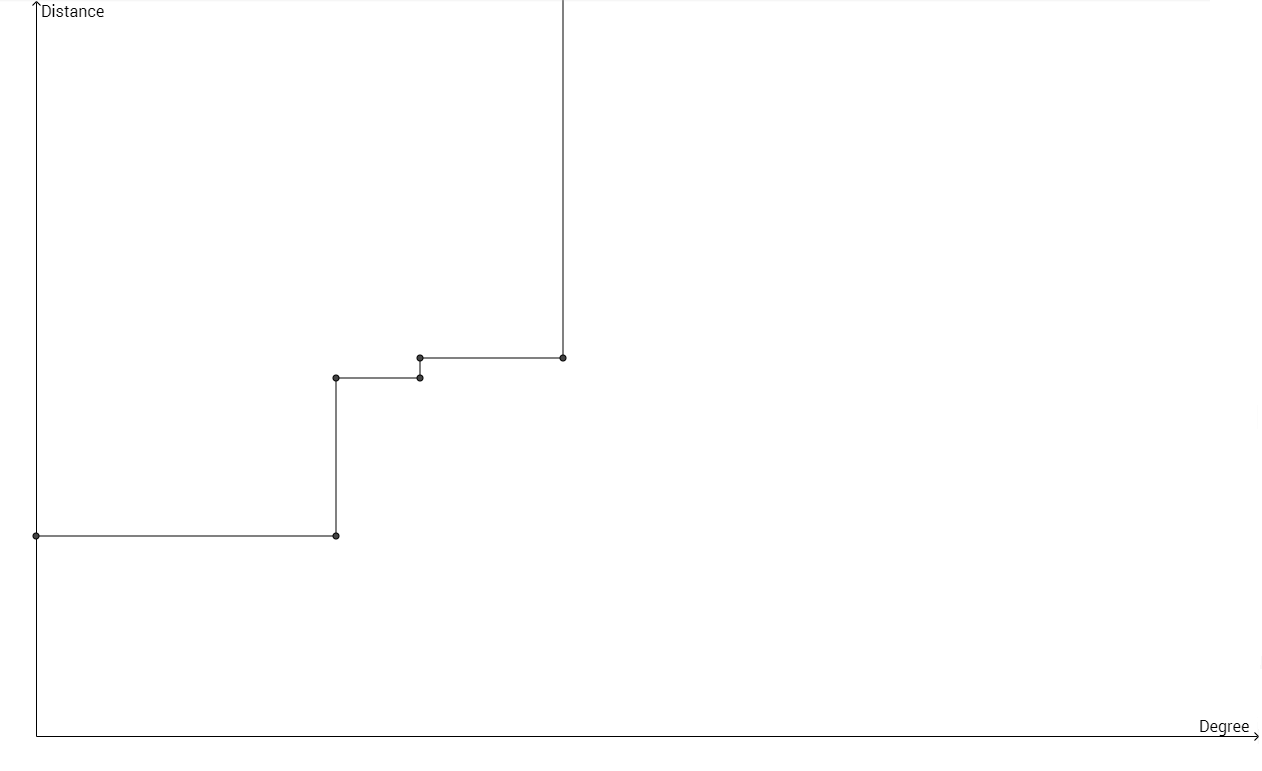
\includegraphics[scale=0.25]{staircase.png}
\end{figure}

In order to compute this set of grades of appearances for each simplex, we use induction. The algorithm is shown below.

\begin{algorithmic}
	\Function{BuildBRComplex}{$d$}
		\State $VGrades \gets \text{GenerateVertexMultigrades}(d)$
		\For{each vertex $k$}
			\State BuildBRSubComplex($d$, $VGrades[k]$, $VGrades$, $\{k\}$)
		\EndFor
	\EndFunction
	
	\Function{BuildBRSubComplex}{$d$, $G$, $VGrades$, $s$}
		\State Store simplex $s$ with grades of appearance $G$.
		\For{vertex $j > \max_{k \in s} k$}
			\State $minDist \gets \max_{k \in s} d(j, k)$
			\State $G' \gets CombineMultigrades(G, VGrades[j], minDist)$
			\State BuildBRSubComplex($d$, $G'$, $VGrades$, $s \cup {j}$)
		\EndFor
	\EndFunction	
\end{algorithmic}

First, we find the grades of appearances for a $0$ simplex, which is just a set with a single point and we store these in the vector of sets $VGrades$. Then, we inductively add vertex by vertex to our simplex. For each additional vertex, we determine the maximum distance between our new vertex and any vertex in the current simplex we are building upon. We can use the information about the grades of appearance of our current simplex, the vertex we are adding, and this minimum distance to compute the grades of appearance for our simplex with this new vertex. The reasoning is shown in the following proposition.

\begin{proposition}
	Let $S_s$ denote the set of all grades of appearance of a simplex $s$, let $S_j$ denote the set of all grades of appearance of a $0$-simplex corresponding to a point $k \not \in s$, and let $d$ be the maximum distance between $k$ and any point in $s$. Let $S'$ be the set of all grades of appearance of the simplex $s \cup \{j\}$. Then $S' = S_s \cap S_j \cap \{(x, y) : y \ge d\}$.
\end{proposition}
\begin{proof}
	Let $(x, y) \in S'$. Since $s \cup {j}$ appears, we know that $s$ and $\{j\}$ both appear and that all lines between $j$ and $s$ appear. Therefore $(x, y) \in S_s \cap S_j \cap \{(x, y): y \ge d\}$.
	
	Let $(x, y) \in S_s \cap S_j \cap \{(x, y): y \ge d\}$. Then all the points in $s \cup \{j\}$ appear and all the lines in $s$ appear as well. Since $y \ge d$, we know that all the lines joining $s$ and $j$ appear and hence the complete graph of $s \cup \{j\}$ appears so $(x, y) \in S'$.
\end{proof}

Now we go over both the algorithm to generate the grades of appearances for a single vertex, and for combining two with a minimum distance parameter. First we explain the algorithm to generate the grades of appearances for a single vertex. The pseudo-code is given below:

\begin{algorithmic}
	\Function{GenerateVertexMultigrades}{$d$}
		\For{each vertex $k$}
			\State $d_k \gets \{d(k, j) : j \neq k\}$
			\State $Grades_k \gets \{(0, 0)\}$
			\State $sort(d_k)$
			\For{$i \gets 0; i < size(d_k); i++$}
				\While{$i + 1 < size(d_k)$ and $d_k[i + 1] = d_k[i]$}
					\State $i++$
				\EndWhile
				\State $Grades_k \gets Grades_k \cup \{(i + 1, d_k(i))\}$
			\EndFor
		\EndFor
	\EndFunction
\end{algorithmic}

The idea is to consider the distinct distances between a vertex $k$ and any other point. We know that each of the defining grades of appearance for the simplex $\{k\}$ must have a $y$ value equal to one of these distinct distances. So for each of these distances $\alpha$, we add the grade of appearance $(|\{j: d(j, k) \le \alpha\}|, \alpha)$. All of these grades of appearances are incomparable because for $\alpha < \alpha'$, we know that there exists a vertex $\ell$ such that $d(\ell, k) = \alpha'$ and hence $|\{j: d(j, k) \le \alpha\}| < |\{j: d(j, k) \le \alpha'\}|$.

Finally, the algorithm to combine multigrades is graphically taking the intersection of two staircases and an upper half plane. In order to do this, we implement a sweeping line algorithm that sweeps from left to right. As it sweeps, for each $x \in \R$ it maintains $\max(\alpha, \min_{(x, y) \in S} y, \min_{(x, y) \in S'} y)$, where $S, S'$ are the set of all grades of appearances of the two staircases. When this maximum changes, we know we have encountered a defining grade of appearance; the maximum increase corresponds to hitting a step in the resultant staircase. In a case of abuse of notation, we let $S, S'$ denote the set of the defining grades of appearance sorted by $x$ value. We also set the $x$ and $y$ value of the ``point'' $S[|S|].x = S[|S|].y = \infty$. The pseudo-code is given below:

\begin{algorithmic}
	\Function{CombineMultigrades}{$S, S', \alpha$}
		\State $G \gets \{\}$
		\State $index1 \gets 0, \index2 \gets 0$
		\State $d = \max(\alpha, S[index1].y, S'[index2].y)$
		\While{$index1 < |S|$ and $index2 < |S'|$}
			\State $minX \gets min(S[index1].x, S'[index2].x)$
			\If{$S[index1].x == minX$}
				\State $index1++$
			\EndIf
			\If{$S'[index2].x == minX$}
				\State $index2++$
			\EndIf
			\State $d' = \max(\alpha, S[index1].y, S'[index2].y)$
			\If{$d' > d$}
				\State $G \gets G \cup \{(minX, d)\}$
				\State $d \gets d'$
			\EndIf
		\EndWhile
	\EndFunction
\end{algorithmic}
\end{document}
